

%\subsection{preamble}

\begin{frame}{what are \emph{you} trying to do with this thing?}

\begin{center}

\includegraphics[width=0.8\textwidth]{computer}
\end{center}
\end{frame}


\begin{frame}{slogans \& scope}

slogans: I will
  \begin{itemize}
  \item \alert{focus on approximating ice flow}
  \item \alert{provide numerical codes that actually work}
  \item \alert{always care about the continuum model}
  \end{itemize}
\medskip

scope: I will cover these
  \begin{itemize}
  \item models

    \begin{itemize}
    \item[$\circ$] shallow ice approximation (SIA) in 2D
    \item[$\circ$] shallow shelf approximation (SSA) in 1D
    \item[$\circ$] mass continuity \& surface kinematical equations
    \end{itemize}

  \item numerical ideas

    \begin{itemize}
    \item[$\circ$] finite difference schemes
    \item[$\circ$] solving algebraic systems from stress balances
    \item[$\circ$] verification
    \end{itemize}
  \end{itemize}
\end{frame}


\begin{comment}
\begin{frame}{outside of scope}

\large\emph{not} \normalsize covered here:\normalsize
\medskip

  \begin{itemize}
  \item Stokes and ``higher order'' flow equations
  \item thermomechanical coupling or polythermal ice
  \item subglacial hydrology/processes
  \item mass balance and snow/firn processes
  \item constitutive relations other than Glen isotropic
  \item grounding lines, calving fronts, ocean interaction
  \item paleo-climate and ``spin-up''
  \item earth deformation under ice sheet load
  \item other numerics: FEM, spectral, multigrid, parallel, \dots
  \item etc.
  \end{itemize}

\end{frame}
\end{comment}

\begin{frame}{notation} 

\begin{center}
  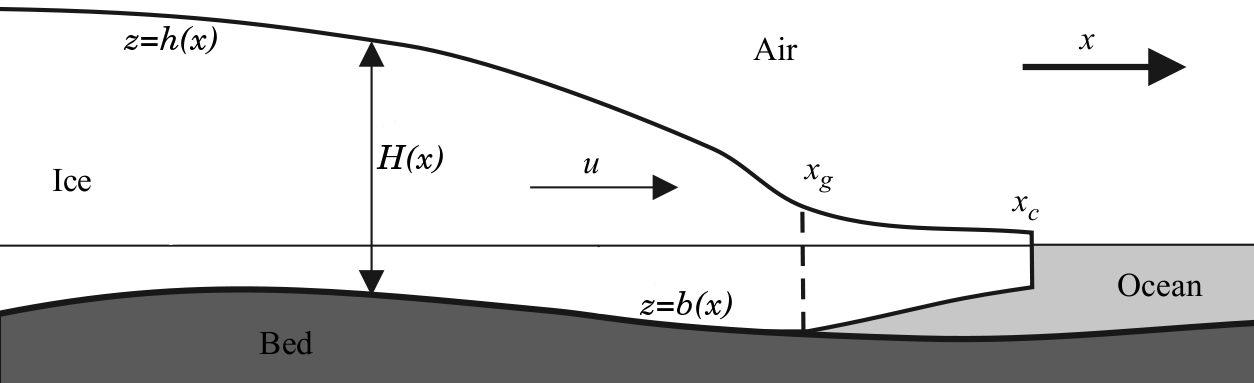
\includegraphics[width=0.9\textwidth]{flowline}

\tiny \emph{figure modified from} Schoof (2007)\nocite{SchoofMarine1}
\end{center}

\scriptsize
  \begin{itemize}
  \item coordinates $t,x,y,z$  (with $z$ vertical, positive upward)
  \item subscripts for partial derivatives $u_x = \partial u/\partial x$
  \item $H=$ ice thickness
  \item $h=$ ice surface elevation
  \item $b=$ bedrock surface elevation
  \item $T=$ temperature
  \item $\mathbf{u}=(u,v,w)=$ ice velocity
  \item $\rho=$ density of ice
  %\item $\rho_w=$ density of ocean water
  \item $g=$ acceleration of gravity
  %\item $n=3$ Glen flow law exponent $=3$
  \item $A=A(T)=$ ice softness in Glen law ($\mathbf{D}_{ij} = A(T) \tau^{n-1} \tau_{ij}$)
  \item \alert{see printed notes for notation}
  \item \alert{please ask about notation!}  (stupid questions impossible)
  \end{itemize}

\end{frame}


\begin{frame}{Matlab/Octave codes}

\begin{itemize}
\item slides and notes are structured around 18 Matlab/Octave codes
\item \dots though only 5 appear in these slides
\item each about 1/2 page of code
\item with rich comments and help files
\item please give them a try!

  \begin{itemize}
  \item[$\circ$] \texttt{.zip} and \texttt{.tar.gz} forms available from memory stick
  \item[$\circ$] and online:

  \bigskip\bigskip\small
  \centerline{\fbox{\url{https://github.com/bueler/karthaus}}}
  
  \end{itemize}
\end{itemize}
\end{frame}


\section[introduction]{introduction: ice flow as viewed from outside glaciology}

\subsection{ice flow equations}

\begin{frame}{ice in glaciers is a \emph{fluid}}

\begin{itemize}
\item<1-> what's a fluid?

\bigskip\bigskip
\item<2> at minimum, we describe fluids by
  \begin{itemize}
  \item[$\circ$] a \emph{density field}\quad $\rho(t,x,y,z)$
  \item[$\circ$] a vector \emph{velocity field}\quad $\mathbf{u}(t,x,y,z)$
  \end{itemize}
\end{itemize}
\end{frame}

\begin{frame}{ice in glaciers is a \emph{fluid} \quad 2}

\begin{itemize}
\item we will assume ice is incompressible
\item if ice fluid were also
  \begin{itemize}
  \item[$\circ$] faster-moving than it actually is, and
  \item[$\circ$] linearly-viscous
  \end{itemize}
  then ice flow would be a ``typical'' fluid like liquid water
\item \dots and one would use the Navier-Stokes equations:
\begin{align*}
\nabla \cdot \mathbf{u} &= 0 &&\text{\emph{incompressibility}} \\
\rho \left(\mathbf{u}_t + \mathbf{u}\cdot\nabla \mathbf{u}\right) &= -\nabla p + \nabla \cdot \tau_{ij} + \rho \mathbf{g} &&\text{\emph{stress balance}} \\
2 \nu \mathbf{D}_{ij} &= \tau_{ij} &&\text{\emph{linear flow law}}
\end{align*}

\bigskip
\item this is the main \emph{continuum model} for fluid dynamics
\item stress balance equation is ``$m a = F$''
\end{itemize}
\end{frame}


\begin{frame}{\emph{hmmm} \dots \emph{does not sound like glaciology to me!}}

\begin{itemize}
\item \alert{yes}, numerical ice sheet flow modelling is ``computational fluid dynamics''
  \begin{itemize}
  \item[$\circ$] it's large-scale like atmosphere and ocean
  \item[$\circ$] \dots\, but it is a weird one
  \end{itemize}
\item consider what makes ocean flow modeling exciting:
  \begin{itemize}
  \item[$\circ$] coriolis force
  \item[$\circ$] density/salinity stratification
  \item[$\circ$] convection
  \item[$\circ$] turbulence
  \end{itemize}
\item \dots\, none of these are relevant to ice flow
\item so what could be interesting about the flow of slow, cold, laminar, old ice?
  \begin{itemize}
  \item[$\circ$] it's \emph{ice dynamics!}
  \end{itemize}
\end{itemize}
\end{frame}


\begin{frame}{ice is a slow, shear-thinning fluid}

\begin{itemize}
\item but \emph{our} fluid is

\smallskip
  \begin{tabular}{lc}
  ``\emph{slow}''\,: & $\rho \left(\mathbf{u}_t + \mathbf{u}\cdot\nabla \mathbf{u}\right) \approx 0$ \\
  \emph{non-Newtonian}\,: & viscosity $\nu$ is not constant
  \end{tabular}

\bigskip
\item slow:
  $$\rho \left(\mathbf{u}_t + \mathbf{u}\cdot\nabla \mathbf{u}\right) \approx 0 \qquad \iff \qquad \begin{pmatrix} \text{forces of inertia} \\ \text{are neglected} \end{pmatrix}$$

\medskip
\item non-Newtonian in a ``shear-thinning'' way
  \begin{itemize}
  \item[$\circ$] higher strain rates means lower viscosity
  \end{itemize}

\bigskip
\item so the standard ``full'' model is power-law ($n=3$) \alert{Stokes}:
\begin{align*}
\nabla \cdot \mathbf{u} &= 0 &&\text{\emph{incompressibility}} \\
0 &= - \nabla p + \nabla \cdot \tau_{ij} + \rho\, \mathbf{g} &&\text{\emph{force balance}} \\
\mathbf{D}_{ij} &= A \tau^2 \tau_{ij} &&\text{\emph{Glen flow law}}
\end{align*}

\end{itemize}
\end{frame}


\begin{frame}{``slow'' means no memory of velocity (i.e.~momentum)}

\begin{itemize}
\item a time-stepping ice sheet code \dots
  \begin{itemize}
  \item[$\circ$] recomputes the full velocity field at every time step, and
  \item[$\circ$] does not require velocity from the previous step
  \end{itemize}

\medskip
\item because the model needs no memory of previous velocity,

\smallskip
\emph{velocity is a ``diagnostic'' output of ice flow models}

\bigskip
\item with BIG apologies to Dylan:

\smallskip
\emph{to be a weatherman you've got to know which way the wind blows \,\dots\, but don't
expect that from a glaciologist}
\end{itemize}
\end{frame}


\subsection{slab-on-a-slope}

\begin{frame}{plane flow Stokes}

\begin{itemize}
\item recall the power-law Stokes model:
\begin{align*}
\nabla \cdot \mathbf{u} &= 0 &&\text{\emph{incompressibility}} \\
0 &= - \nabla p + \nabla \cdot \tau_{ij} + \rho\, \mathbf{g} &&\text{\emph{force balance}} \\
\mathbf{D}_{ij} &= A \tau^2 \tau_{ij} &&\text{\emph{Glen flow law}}
\end{align*}

\bigskip
\item now work in a $x,z$ \alert{plane}
  \begin{itemize}
  \item[$\circ$] like the centerline of a glacier
  \item[$\circ$] or in a cross-flow plane
  \end{itemize}

\item notation on next slide:
  \begin{itemize}
  \item[$\circ$] $x,z$ subscripts are partial derivatives
  \item[$\circ$] $\tau_{13}$ is the ``vertical'' shear stress
  \item[$\circ$] $\tau_{11}$ and $\tau_{33}=-\tau_{11}$ are (deviatoric) longitudinal stresses 
  \end{itemize}
\end{itemize}
\end{frame}

\begin{frame}{plane flow Stokes  \quad 2}

\begin{itemize}
\item in the $x,z$ plane flow case the Stokes equations say
\begin{empheq}[]{align}
u_x + w_z &= 0 &&\text{\emph{incompressibility}}\notag \\
p_x &= \tau_{11,x} + \tau_{13,z} &&\text{\emph{stress balance} ($x$)} \notag \\
p_z &= \tau_{13,x} - \tau_{11,z} - \rho g &&\text{\emph{stress balance} ($z$)} \notag \\
u_x &= A \tau^2 \tau_{11} &&\text{\emph{flow law} (diagonal)}\notag \\
u_z + w _x &= 2 A \tau^2 \tau_{13} &&\text{\emph{flow law} (off-diagonal)} \notag
\end{empheq}
\item we have five equations in five unknowns ($u,w,p,\tau_{11},\tau_{13}$)
\item complicated enough \dots what about in a simplified situation?
\end{itemize}
\end{frame}


\begin{frame}{slab-on-a-slope}

\vspace{-0.05in}
\small

\begin{columns}

\begin{column}{0.5\textwidth}
\begin{itemize}
\item suppose we have
  \begin{itemize}
  \item[$\circ$] constant thickness and 
  \item[$\circ$] tilted bed
  \end{itemize}
\item rotated coordinates give:
  $$\mathbf{g} = g \sin\theta\, \hat x - g \cos \theta \,\hat z$$
\item so $p_x,p_z$ equations are now:
\begin{align}
p_x &= \tau_{11,x} + \tau_{13,z} + \rho g \sin\theta \notag \\
p_z &= \tau_{13,x} - \tau_{11,z} - \rho g \cos\theta \notag
\end{align}
\end{itemize}
\end{column}

\begin{column}{0.5\textwidth}
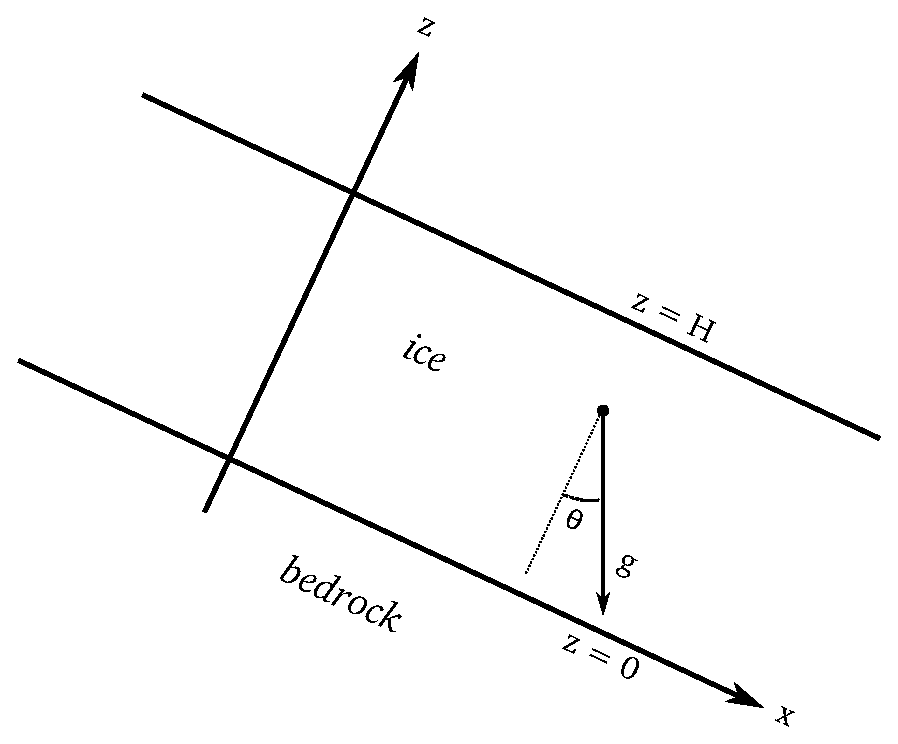
\includegraphics[width=1.0\textwidth]{slab}
\end{column}

\end{columns}

\begin{itemize}
\item for an infinite \alert{slab-on-a-slope} there is \emph{no variation in} $x$
\item the equations simplify:
\small
\begin{align}
w_z &\stackrel{1}{=} 0 &   0 &= \tau_{11} \notag \\
p_z &\stackrel{2}{=} - \rho g \cos\theta &   u_z &= 2 A \tau^2 \tau_{13} \notag \\
\tau_{13,z} &\stackrel{3}{=} - \rho g \sin\theta \notag
\end{align}
\normalsize
\end{itemize}
\end{frame}


\begin{frame}{slab-on-a-slope 2}

\begin{itemize}
\item add some boundary conditions:
	$$u(\text{base})=u_0, \qquad w(\text{base})=0, \qquad p(\text{surface})=0$$
\item by integrating 1,2,3 vertically, get (see figure):
  $$w=0, \qquad p = \rho g \cos\theta (H-z), \qquad \tau_{13} = \rho g \sin\theta (H-z)$$
\item and from ``$u_z = 2 A \tau^2 \tau_{13}$'' get \alert{velocity formula}:
\vspace{-0.05in}
\begin{align*}
u(z) &= u_0 + 2 A (\rho g \sin\theta)^3 \int_0^z (H-z')^3\,dz' \\
     &= u_0 + \frac{1}{2} A (\rho g \sin\theta)^3  \left(H^4 - (H-z)^4\right)
\end{align*}
\end{itemize}

\vspace{-15mm}
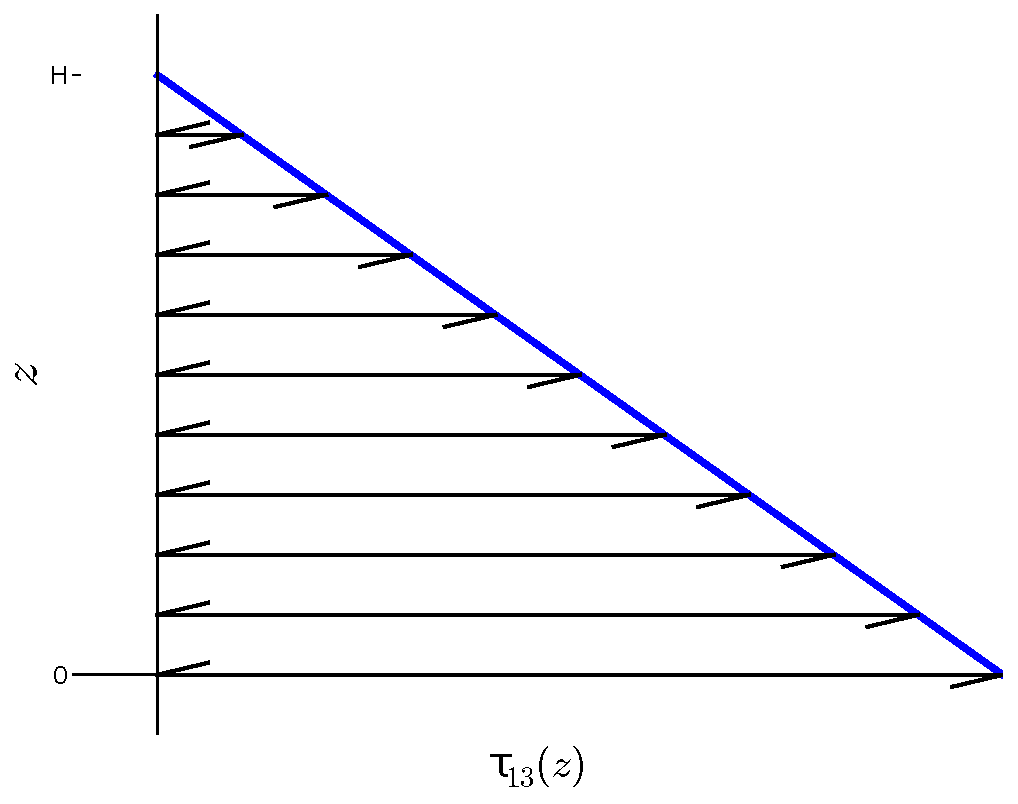
\includegraphics[width=0.5\textwidth]{slabshear}
\end{frame}


\begin{frame}{slab-on-a-slope 3}

\begin{columns}
\begin{column}{0.6\textwidth}
\begin{itemize}
\item do we believe these equations?
\item velocity formula on last slide gives figure below
\item compare to observations at right
\end{itemize}
\begin{center}
% NOT preserving aspect ratio
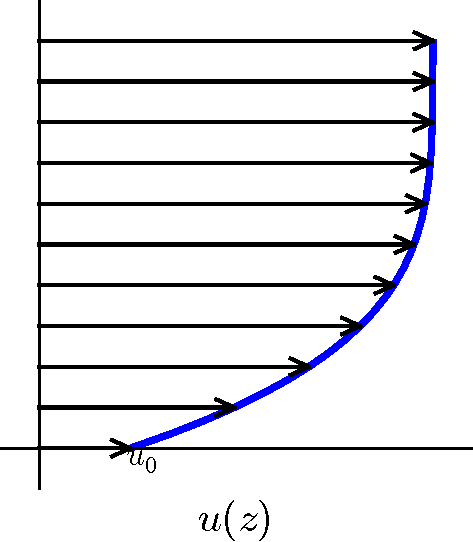
\includegraphics[width=0.6\textwidth,height=0.5\textheight]{slabvel}
\end{center}
\end{column}

\begin{column}{0.4\textwidth}
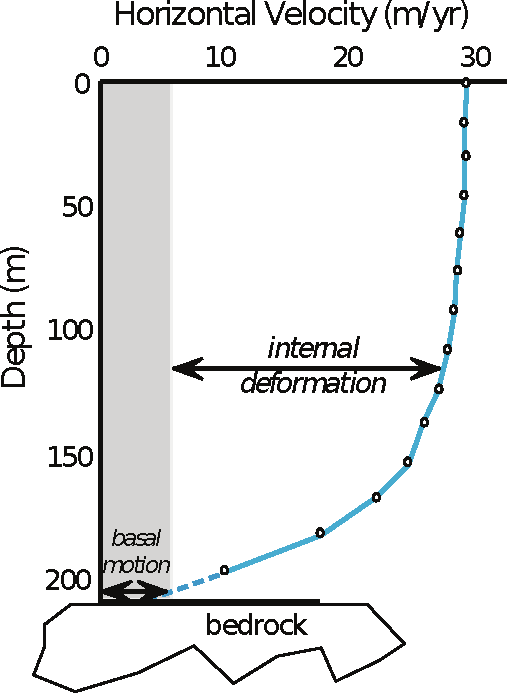
\includegraphics[width=1.0\textwidth]{athabasca_deform}

\medskip
\scriptsize
Velocity profile of the Athabasca Glacier, Canada, derived from inclinometry (Savage and Paterson, 1963)\nocite{SavagePaterson}
\end{column}
\end{columns}
\end{frame}


\begin{frame}{mass continuity}

\begin{itemize}
\item now we know the velocity $u$ \qquad \dots so what?
\item suppose, instead of slab-on-a-slope, that our ice flow has \alert{variable thickness} $H(t,x)$
\item compute the vertical average of velocity:
	$$\bar U(t,x) = \frac{1}{H}\int_0^{H} u(t,x,z)\,dz$$
\end{itemize}
\end{frame}


\begin{frame}{mass continuity \quad 2}

\begin{columns}
\begin{column}{0.6\textwidth}
\begin{itemize}
\item $M(x)$ is climatic mass balance
\item consider change of area $A$ in figure:
	$$\frac{dA}{dt} \stackrel{\ast}{=} \int_{x_1}^{x_2} M(x)\,dx + \bar U_1 H_1 - \bar U_2 H_2 \phantom{foobar}$$
\item assume width $\Delta x=x_2-x_1$ is small so $A\approx \Delta x\, H$
\end{itemize}
\end{column}
\begin{column}{0.4\textwidth}

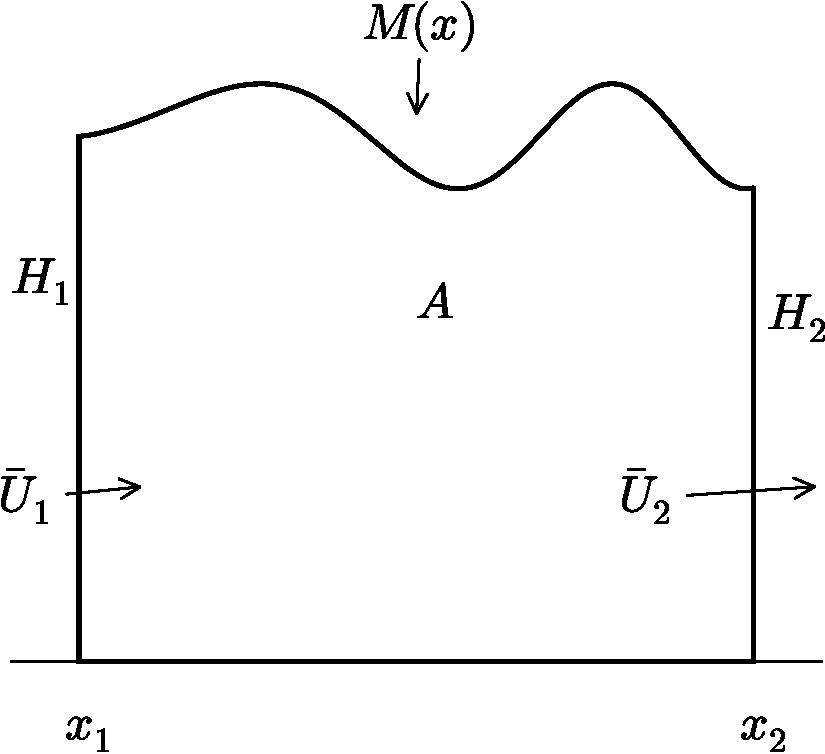
\includegraphics[width=1.0\textwidth]{slabmasscontfig}

\vspace{0pt}
\end{column}
\end{columns}

\bigskip
\begin{itemize}
\item divide eqn $\ast$ by $\Delta x$ and get
   $$H_t = M - \left(\bar U H\right)_x$$
\item this is a \emph{mass continuity equation}
\item ``area'' in 2D becomes ``volume'' in 3D
\end{itemize}
\end{frame}


\begin{frame}{combine equations so far \dots}

\begin{itemize}
\item from slab-on-slope velocity formula in $u_0=0$ case,
\begin{align*}
\bar u H &= \int_0^H \frac{1}{2} A (\rho g \sin\theta)^3  \left(H^4 - (H-z)^4\right)\,dz \\
	&= \frac{2}{5} A (\rho g \sin\theta)^3 H^5
\end{align*}
\item note $\sin \theta \approx \tan\theta = - h_x$
\item combine with mass continuity $H_t = M - \left(\bar u H\right)_x$ to get:
  $$H_t = M + \left(\frac{2}{5} (\rho g)^5 A H^5 |h_x|^2 h_x\right)_x$$

\medskip
\item this is rough explanation of ``shallow ice approximation''
\item \dots which will be our first numerically-solved ice flow model!
\end{itemize}
\end{frame}